\documentclass{beamer}

\usepackage[brazil]{babel}
\usepackage[alf]{abntex2cite}
\usepackage{graphicx,hyperref,ru,url}
\usepackage[T1]{fontenc}
\usepackage[utf8]{inputenc}

% The title of the presentation:
%  - first a short version which is visible at the bottom of each slide;
%  - second the full title shown on the title slide;
\title[Cálculo Variacional]{Cálculo Variacional}

% Optional: a subtitle to be dispalyed on the title slide
%\subtitle{Apenas um subtítulo}

% The author(s) of the presentation:
%  - again first a short version to be displayed at the bottom;
%  - next the full list of authors, which may include contact information;
\author[Eduardo Oliveira]{Eduardo José de Oliveira}

% The institute:
%  - to start the name of the university as displayed on the top of each slide
%    this can be adjusted such that you can also create a Dutch version
%  - next the institute information as displayed on the title slide
\institute[Universidade Estadual de Goiás]{
	UNIVERSIDADE ESTADUAL DE GOIÁS\\
  	Câmpus Anápolis de Ciências Exatas e Tecnológicas Henrique Santillo \\
  	Licenciatura Em Matemática}

% Add a date and possibly the name of the event to the slides
%  - again first a short version to be shown at the bottom of each slide
%  - second the full date and event name for the title slide
\date[2019]{2019}

\newtheorem{definicao}{Definição}

\newcommand{\makesubtitleframe}[1]{
	{
		\usebackgroundtemplate{
\includegraphics[width=\paperwidth]{ueg_background_title}}
		\begin{frame}
			\vfill
			\begin{center}
				{\Huge\usebeamercolor[white]{}#1}
			\end{center}
			\vfill
		\end{frame}
	}
}

\begin{document}

	\begin{frame}[plain]
	  \titlepage
	\end{frame}


\begin{frame}
  %\frametitle{Índice}
  \tableofcontents
\end{frame}

% Section titles are shown in at the top of the slides with the current section 
% highlighted. Note that the number of sections determines the size of the top 
% bar, and hence the university name and logo. If you do not add any sections 
% they will not be visible.
\section{Introdução}

\begin{frame}
  \frametitle{Introdução}

  	O problema pertinente ao cálculo variacional é o de encontrar uma função diferenciável até segunda ordem $y=y(x)$ satisfazendo $y(x_1)=y_1$ e $y(x_2)=y_2$, com $x_1$, $x_2$, $y_1$ e $y_2$ dados, minimizando ou maximizando a integral
	$$
		\int_{x_1}^{x_2} f(x,y,y')dx\text{.}
	$$
\end{frame}

\section{História}
\makesubtitleframe{História}

\begin{frame}
  \frametitle{Máximos e Mínimos}

	\begin{itemize}
		\item Pierre de Fermat em 1629.
		\item Comparações entre $f(x)$ e $f(x+E)$ próximo de máximos ou mínimos.
		\item Considerar a divisão $\frac{f(x+E)-f(x)}{E}$.
		\item Após a divisão, considerar $E=0$.
		\item Por último, igualar o resultado a $0$, encontrando as abscissas dos máximos ou mínimos.
	\end{itemize}

\end{frame}

\begin{frame}
	\frametitle{Problema da Braquistócrona}
	\begin{itemize}
		\item Formulado por Johann Bernoulli em 1969, pode ser apresentado como:
		\begin{block}{Problema da Braquistócrona}
			Sejam $A$ e $B$ dois pontos dados em um plano vertical. O problema da braquistócrona consiste em encontrar a curva que uma partícula M precisa descrever para sair de A e chegar em B no menor tempo possível, somente sob a ação da força da gravidade \cite[p. 3]{calcvar}.
		\end{block}
		
		\item Solução de Jacob Bernoulli (1697) apresenta o aspecto da curva variável.
		
		\item Euler e Lagrange.
	\end{itemize}
\end{frame}

\section{Cálculo Variacional}
\makesubtitleframe{Cálculo Variacional}

\begin{frame}
	\frametitle{Relembrando o problema}
	Deseja-se encontrar uma função diferenciável até segunda ordem $y=y(x)$ satisfazendo $y(x_1)=y_1$ e $y(x_2)=y_2$, com $x_1$, $x_2$, $y_1$ e $y_2$ dados, minimizando ou maximizando a integral
	\begin{equation}
		\int_{x_1}^{x_2} f(x,y,y')dx\text{.}
		\label{eqn:def_calcvar}
	\end{equation}
\end{frame}

\begin{frame}
	\frametitle{Funções Aproximadoras}
	\begin{definicao}
		Uma família de funções aproximadoras é definida como
		$$Y(x)=y(x)+\varepsilon \eta (x)\text{,}$$
		onde $\eta (x)$ é uma função diferenciável arbitrária para a qual $\eta (x_1)=\eta (x_2)=0$. O número $\varepsilon$ é o parâmetro da família.
		
		Sua derivada pode ser escrita como
		$$Y'(x)=y'(x)+\varepsilon \eta '(x)\text{.}$$
	\end{definicao}
\end{frame}

{
\usebackgroundtemplate{}
	\begin{frame}
		\begin{figure}
			\caption{Representação gráfica das funções aproximadoras.}
			\begin{center}
				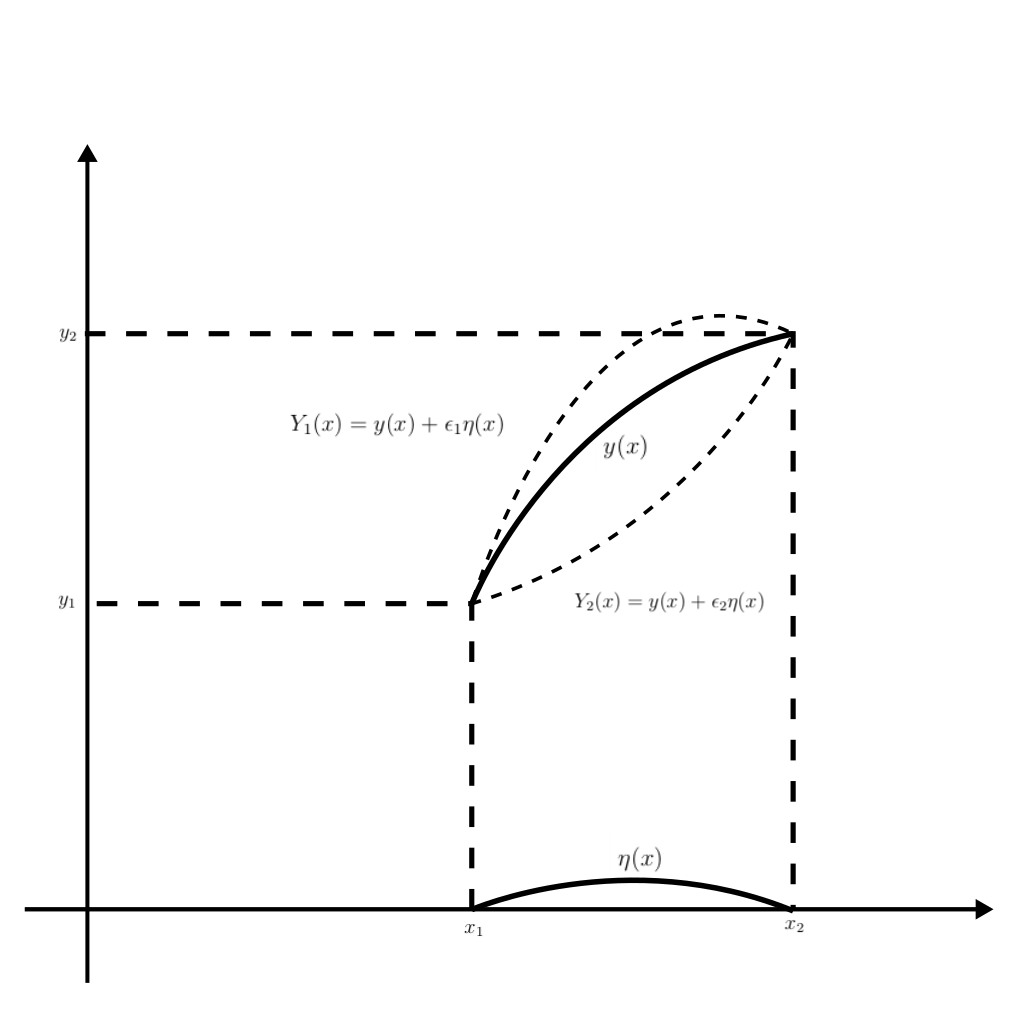
\includegraphics[scale=0.25]{figura_001}\par
				{\small Fonte: Elaborada pelo autor, 2019}
			\end{center}
			\label{fig:func_approx}
		\end{figure}
	\end{frame}
}
	
\begin{frame}
	\frametitle{Reescrevendo o Problema}
	Pode-se reescrever a integral \eqref{eqn:def_calcvar} utilizando as funções aproximadoras, em função de $\varepsilon$, então
	\begin{equation}
		\label{eqn:int_funcional_approx}
		I(\varepsilon)=\int_{x_1}^{x_2}f(x, Y, Y')dx\text{.}
	\end{equation}
	
	Para encontrar a função $y(x)$ que maximiza ou minimiza a integral escrita com as funções aproximadoras \eqref{eqn:int_funcional_approx}, deve-se fazer
	$$I'(\varepsilon)=0\text{,}$$
	e, considerando que quando $\varepsilon=0$, as integrais \eqref{eqn:def_calcvar} e \eqref{eqn:int_funcional_approx} fornecem os mesmos maximos e mínimos, é necessário que
	$$I'(0)=0\text{.}$$
\end{frame}

\begin{frame}
	\frametitle{Equação de Euler-Lagrange}
	
	Desenvolvendo os cálculos, chega-se a equação diferencial parcial chamada de Equação de \textbf{Euler-Lagrange}:
	\begin{equation}
		\label{eqn:cap_calcvar_euler_lagrange}
		\frac{\partial f}{\partial y} - \frac{d}{dx} \left ( \frac{\partial f}{\partial y'} \right )=0 \text{.}
	\end{equation}
	
	A equação \eqref{eqn:cap_calcvar_euler_lagrange} permite encontrar a função $y(x)$ que maximiza ou minimiza a integral \eqref{eqn:def_calcvar}.
\end{frame}

\nocite{boyer}
\nocite{hist_still}
\nocite{hist_courant}
\nocite{mefassan}

\section{Referências}
\begin{frame}
	\frametitle{Referências}
	\bibliography{references}
\end{frame}

\end{document}
